\section{正则化方法}
\label{sec:ls-truncated-svd-ridge}

上一节表明，数据误差沿小奇异值方向被放大$1/\sigma_i$倍。QR等正交算法只能避免在问题本身的敏感度之外再损失精度，改变不了这种放大。本节换一种做法：主动修改求解目标，用一部分拟合误差换取解的稳定。

修改目标有两种方式，分两小节讨论。岭回归与Tikhonov正则化在目标中加入惩罚项，连续地压低敏感方向；谱截断正则化直接舍弃小奇异值方向。每小节先从要解的问题出发说明新目标及其在奇异方向上的作用，再在小例子上逐步执行算法，最后分析误差与代价。由于目标已经改变，算出的是新目标的解，不能把它当作原问题更准确的解。

\subsection{岭回归与Tikhonov正则化}
\label{sec:ls-regularized-ls}

\subsubsection{主要思想}

\paragraph{在目标中加入惩罚}
最小二乘只要求拟合。设计矩阵接近秩亏时，拟合几乎同样好的系数可以相差很远，其中往往有分量很大、彼此抵消的一组。要排除这样的系数，就要在目标中同时衡量系数的大小。对$\lambda>0$，\term{岭回归}（ridge regression）求解
\begin{equation}
 \min_{\bm x}\ \lVert\bm A\bm x-\bm b\rVert_2^2+\lambda\lVert\bm x\rVert_2^2 .
 \label{eq:ls-ridge-objective}
\end{equation}
第二项惩罚系数的长度：拟合同样好的两个解中，目标偏向长度较小的一个；$\lambda$越大，这种偏向越强。

惩罚也可以作用在其他希望压小的量上，例如相邻分量之差。取惩罚矩阵$\bm\Gamma\in\mathbb R^{p\times d}$，目标改为
\begin{equation}
 \lVert\bm A\bm x-\bm b\rVert_2^2+\lambda\lVert\bm\Gamma\bm x\rVert_2^2 ,
 \label{eq:ls-tikhonov-objective}
\end{equation}
称为\term{Tikhonov正则化}（Tikhonov regularization）\scite{math-hansen2008regtools}。岭回归是$\bm\Gamma=\bm I$的情形；取$\bm\Gamma=[\,1\ \ -1\,]$则惩罚两个分量之差。文献中惩罚矩阵常记作$\bm L$；本部分的$\bm L$已用于表示矩阵的严格下三角部分（第~\ref{sec:ls-matrix-splitting}节），所以这里改记为$\bm\Gamma$。

\paragraph{化为增广最小二乘}
新目标是两个平方长度之和。两个向量平方长度之和，等于把它们上下堆叠成一个向量后的平方长度。先在下面的小例子上按元素看这一点：
\[
 \bm A=\operatorname{diag}(3,1),\qquad \bm b=\begin{bmatrix}3\\1\end{bmatrix},\qquad \bm\Gamma=\bm I,\qquad \lambda=1 .
\]
这时岭回归的目标是
\[
 (3x_1-3)^2+(x_2-1)^2+x_1^2+x_2^2 .
\]
前两项来自拟合，后两项来自惩罚。四项合起来恰是向量$(3x_1-3,\ x_2-1,\ x_1,\ x_2)^\top$的平方长度，而这个向量可以写成
\[
 \begin{bmatrix}3x_1-3\\x_2-1\\x_1\\x_2\end{bmatrix}
 =\begin{bmatrix}3&0\\0&1\\1&0\\0&1\end{bmatrix}\begin{bmatrix}x_1\\x_2\end{bmatrix}
 -\begin{bmatrix}3\\1\\0\\0\end{bmatrix}.
\]
所以这个岭回归就是一个四行两列的普通最小二乘问题：惩罚在原数据下方添了两行，对应的右端为零。

一般情形完全相同。由$\lambda\lVert\bm\Gamma\bm x\rVert_2^2=\lVert\sqrt\lambda\,\bm\Gamma\bm x-\bm0\rVert_2^2$，Tikhonov正则化是一个\term{增广最小二乘}（augmented least squares）问题
\begin{equation}
 \min_{\bm x}\lVert\tilde{\bm A}\bm x-\tilde{\bm b}\rVert_2^2,\qquad
 \tilde{\bm A}=\begin{bmatrix}\bm A\\ \sqrt\lambda\,\bm\Gamma\end{bmatrix},\quad
 \tilde{\bm b}=\begin{bmatrix}\bm b\\ \bm0\end{bmatrix}.
 \label{eq:ls-augmented-system}
\end{equation}
在计算上，惩罚只是在原数据下方增加了$p$行：每一行要求$\sqrt\lambda$倍的线性组合$(\bm\Gamma\bm x)_i$接近零。

\paragraph{解的存在与唯一}
既然新目标是一个普通最小二乘问题，第~\ref{sec:ls-ordinary-ls}节关于解集的结论就可以直接搬过来。

\begin{theorem}[Tikhonov解的存在与唯一]
\label{thm:ls-tikhonov-existence-uniqueness}
设$\bm A\in\mathbb R^{m\times d}$，$\bm\Gamma\in\mathbb R^{p\times d}$，$\lambda>0$。Tikhonov目标的极小点恰为方程
\begin{equation}
 (\bm A^\top\bm A+\lambda\bm\Gamma^\top\bm\Gamma)\bm x=\bm A^\top\bm b
 \label{eq:ls-tikhonov-normal-equation}
\end{equation}
的解，这样的解总存在；解唯一当且仅当
\begin{equation}
 \ker\bm A\cap\ker\bm\Gamma=\{\bm0\}.
 \label{eq:linear-algebra-tikhonov-common-nullspace}
\end{equation}
特别地，岭回归对任意$\bm A$都有唯一解。
\end{theorem}
\begin{proof}
目标等于增广问题~\eqref{eq:ls-augmented-system}。由第~\ref{sec:ls-ordinary-ls}节，增广残差与$\tilde{\bm A}$的列空间正交的点就是极小点，即正规方程
\[
 \tilde{\bm A}^\top\tilde{\bm A}\bm x=\tilde{\bm A}^\top\tilde{\bm b}
\]
的解；它总存在，且唯一当且仅当$\ker\tilde{\bm A}=\{\bm0\}$。按分块乘法，
\[
 \tilde{\bm A}^\top\tilde{\bm A}=\bm A^\top\bm A+\lambda\bm\Gamma^\top\bm\Gamma,\qquad \tilde{\bm A}^\top\tilde{\bm b}=\bm A^\top\bm b ,
\]
代入即得上面的方程。

再看唯一性。对任意$\bm x$，
\[
 \bm x^\top(\bm A^\top\bm A+\lambda\bm\Gamma^\top\bm\Gamma)\bm x=\lVert\bm A\bm x\rVert_2^2+\lambda\lVert\bm\Gamma\bm x\rVert_2^2 ,
\]
$\lambda>0$时它为零当且仅当$\bm A\bm x=\bm0$且$\bm\Gamma\bm x=\bm0$，所以$\ker\tilde{\bm A}=\ker\bm A\cap\ker\bm\Gamma$。岭回归中$\ker\bm I=\{\bm0\}$。
\end{proof}

一般的$\bm\Gamma$未必满足条件~\eqref{eq:linear-algebra-tikhonov-common-nullspace}。取$\bm A=\bm\Gamma=[\,1\ \ -1\,]$，方向$(1,1)^\top$既不影响拟合也不受惩罚，无论$\lambda$多大，两个分量的共同水平都定不下来。

还要注意，目标中的平方不能去掉。无惩罚时，最小化残差范数与最小化它的平方是同一个问题；加入惩罚以后，最小化$\lVert\bm A\bm x-\bm b\rVert_2+\lambda\lVert\bm x\rVert_2$是另一个问题，不能与式~\eqref{eq:ls-ridge-objective}互换。

\paragraph{奇异方向上的滤波}
惩罚究竟压低了哪些方向，可以在奇异坐标中逐个看清。设$\bm A$的秩为$r$，正奇异值与奇异向量为$\sigma_i,\bm u_i,\bm v_i$，记右端在第$i$个左奇异方向上的分量为
\begin{equation}
 c_i=\bm u_i^\top\bm b .
 \label{eq:ls-rhs-singular-coefficients}
\end{equation}

\begin{theorem}[岭回归的滤波因子]
\label{thm:ls-ridge-filter-factors}
设$\lambda>0$，$\bm x_\lambda$为岭回归~\eqref{eq:ls-ridge-objective}的解，则
\begin{equation}
 \bm x_\lambda=\sum_{i=1}^r f_i\,\frac{c_i}{\sigma_i}\,\bm v_i,\qquad
 f_i=\frac{\sigma_i^2}{\sigma_i^2+\lambda}\in(0,1).
 \label{eq:matrix-analysis-ridge-filter-factor}
\end{equation}
每个方向的增益$\sigma_i/(\sigma_i^2+\lambda)$不超过$1/(2\sqrt\lambda)$。残差平方为
\begin{equation}
 \lVert\bm b-\bm A\bm x_\lambda\rVert_2^2=\lVert(\bm I-\bm A\bm A^\dagger)\bm b\rVert_2^2+\sum_{i=1}^r(1-f_i)^2c_i^2,
 \label{eq:ls-ridge-residual}
\end{equation}
它随$\lambda$增大而不减，$\lVert\bm x_\lambda\rVert_2$随$\lambda$增大而不增，且$\lambda\to0^+$时$\bm x_\lambda\to\bm A^\dagger\bm b$。
\end{theorem}
\begin{proof}
把右奇异向量补成$\mathbb R^d$的标准正交基$\bm v_1,\ldots,\bm v_d$，令$\bm x=\sum_iz_i\bm v_i$。由$\bm A\bm v_i=\sigma_i\bm u_i$（$i\leq r$）与$\bm A\bm v_i=\bm0$（$i>r$），并把$\bm b$分成列空间内的$\sum_{i\leq r}c_i\bm u_i$与正交补中的$(\bm I-\bm A\bm A^\dagger)\bm b$，目标化为
\[
 \begin{aligned}
 &\lVert(\bm I-\bm A\bm A^\dagger)\bm b\rVert_2^2\\
 &\qquad+\sum_{i=1}^r\bigl[(\sigma_iz_i-c_i)^2+\lambda z_i^2\bigr]+\lambda\sum_{i>r}z_i^2 .
 \end{aligned}
\]
各坐标互不耦合，可以逐个配方：
\[
 \begin{aligned}
 (\sigma_iz_i-c_i)^2+\lambda z_i^2
 &=(\sigma_i^2+\lambda)\Bigl(z_i-\frac{\sigma_ic_i}{\sigma_i^2+\lambda}\Bigr)^2\\
 &\quad+\frac{\lambda c_i^2}{\sigma_i^2+\lambda},
 \end{aligned}
\]
所以
\[
 z_i=\frac{\sigma_ic_i}{\sigma_i^2+\lambda}\qquad(i\leq r),
\]
而零空间坐标只受惩罚，取$z_i=0$（$i>r$）。这就是式~\eqref{eq:matrix-analysis-ridge-filter-factor}。

增益界来自$\sigma_i^2+\lambda\geq2\sigma_i\sqrt\lambda$。由$\bm A\bm x_\lambda=\sum_if_ic_i\bm u_i$，残差在$\operatorname{range}\bm A$内的分量为$\sum_i(1-f_i)c_i\bm u_i$，与列空间外的分量正交，得到残差公式。

$1-f_i=\lambda/(\sigma_i^2+\lambda)$随$\lambda$增大，$f_i/\sigma_i$随$\lambda$减小，故两个单调性成立；$\lambda\to0^+$时$f_i\to1$，极限为第~\ref{sec:ls-pseudoinverse}节的$\bm A^\dagger\bm b$。
\end{proof}

与最小范数解$\bm A^\dagger\bm b=\sum_i(c_i/\sigma_i)\bm v_i$相比，岭回归在每个方向上多乘了一个\term{滤波因子}（filter factor）$f_i$。回到前面的小例子：$\bm A=\operatorname{diag}(3,1)$的奇异向量就是坐标向量，$\sigma_1=3$，$\sigma_2=1$，$c_1=3$，$c_2=1$。按分量写出最小范数解的系数、滤波因子与岭回归的系数：
\[
 \begin{aligned}
 &\text{第一个方向：}&& \frac{c_1}{\sigma_1}=1,\qquad f_1=\frac{9}{9+1}=\frac9{10},\qquad f_1\frac{c_1}{\sigma_1}=\frac9{10};\\
 &\text{第二个方向：}&& \frac{c_2}{\sigma_2}=1,\qquad f_2=\frac{1}{1+1}=\frac12,\qquad f_2\frac{c_2}{\sigma_2}=\frac12 .
 \end{aligned}
\]
于是
\[
 \bm x_\lambda=\begin{bmatrix}9/10\\1/2\end{bmatrix}.
\]
两个方向的最小范数系数相同，但奇异值较大的第一个方向只被压低十分之一，奇异值较小的第二个方向被压掉一半。

一般地，伪逆在第$i$个方向的增益$1/\sigma_i$被换成有界的$\sigma_i/(\sigma_i^2+\lambda)$，不再随$\sigma_i\to0$爆炸。$\sigma_i^2\gg\lambda$的方向几乎不变，$\sigma_i^2\ll\lambda$的方向被压低，转折点在$\sigma_i=\sqrt\lambda$：那里$f_i=1/2$，增益达到峰值。上例中$\sqrt\lambda=1=\sigma_2$，第二个方向正好落在转折点上。

图~\ref{fig:ls-ridge-tsvd-filter-factors}画出了两种$\lambda$下的滤波因子与增益：$\lambda$每增大一百倍，转折点就向大奇异值移动一个数量级，增益峰值降为十分之一。

代价是拟合改变了，偏差随之引入。$\lambda$太小，噪声沿小奇异值方向放大；$\lambda$太大，真实信号也被压掉。合适的参数依赖数据误差与任务目标，例如已知误差规模$\epsilon$时取使$\lVert\bm b-\bm A\bm x_\lambda\rVert_2\approx\epsilon$的$\lambda$，或在留出的数据上检验预测效果；不能只因某个参数使计算容易就宣称它最合适。

\begin{figure}[htbp]
 \centering
 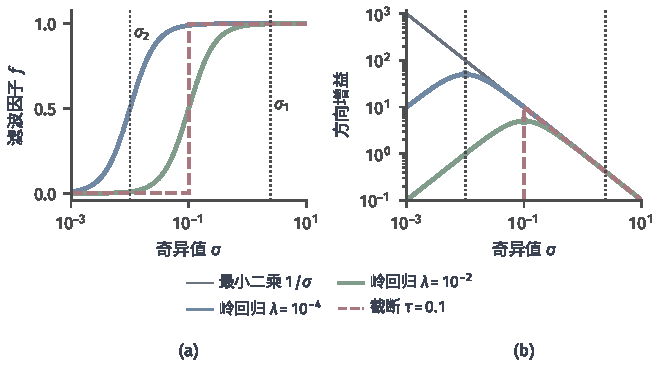
\includegraphics[width=112mm]{figures/01-basic-mathematics/03-vectors-matrices-and-multivariate-functions/matplotlib/c5-ridge-tsvd-filter-factors/figure.pdf}
 \caption{岭回归与截断SVD沿奇异方向的作用。(a)滤波因子：岭回归$f=\sigma^2/(\sigma^2+\lambda)$在$\sigma=\sqrt\lambda$处取$1/2$并连续过渡，截断SVD在阈值$\tau$处由$0$跳到$1$。(b)方向增益：最小二乘为$1/\sigma$，岭回归为$\sigma/(\sigma^2+\lambda)$，圆点是峰值$1/(2\sqrt\lambda)$；截断后小于$\tau$的方向增益为零。竖虚线是示例~\ref{ex:ls-tsvd-steps}中矩阵的两个奇异值。}
 \label{fig:ls-ridge-tsvd-filter-factors}
\end{figure}

\subsubsection{算法实现}
先区分两件事。第~\ref{sec:ls-qr-method}节的正交算法改善的是同一问题的计算过程；正则化则主动修改了问题，以控制敏感性。修改后的问题是增广最小二乘~\eqref{eq:ls-augmented-system}，所以首选的计算路线是对增广矩阵作QR分解，它适用于任意$\bm\Gamma$。下面写出这条路线的变量、输入与预处理和计算步骤，并在主要思想的小例子上执行。

\begin{example}[增广QR求岭回归]
\label{ex:ls-ridge-augmented-qr}
本例取主要思想中的教学例：
\[
 \bm A=\begin{bmatrix}3&0\\0&1\end{bmatrix},\qquad
 \bm b=\begin{bmatrix}3\\1\end{bmatrix},\qquad
 \bm\Gamma=\bm I,\qquad \lambda=1 .
\]
无惩罚时方程相容，解为$(1,1)^\top$。下面的逐步执行都在这个例子上进行。
\end{example}

\paragraph{变量}
\begin{itemize}
 \item $\tilde{\bm A}\in\mathbb R^{(m+p)\times d}$、$\tilde{\bm b}\in\mathbb R^{m+p}$：增广矩阵与增广右端。
 \item $\bm Q\in\mathbb R^{(m+p)\times d}$、$\bm R\in\mathbb R^{d\times d}$：$\tilde{\bm A}$的经济型QR因子，$\bm Q$的列标准正交，$\bm R$为对角元为正的上三角矩阵。
 \item $\bm g\in\mathbb R^d$：变换后的右端$\bm Q^\top\tilde{\bm b}$。
 \item $\bm x\in\mathbb R^d$：正则化解$\bm x_\lambda$。
 \item $\bm r\in\mathbb R^m$：原残差$\bm b-\bm A\bm x$；另报告惩罚量$\lVert\bm\Gamma\bm x\rVert_2$。
\end{itemize}

\paragraph{输入与预处理}
输入$\bm A,\bm b,\bm\Gamma,\lambda$。先核对$\bm A$与$\bm\Gamma$的列数相同、$\bm b$的长度等于$\bm A$的行数，再把增广矩阵与增广右端构造为
\[
 \tilde{\bm A}=\begin{bmatrix}\bm A\\ \sqrt\lambda\,\bm\Gamma\end{bmatrix},\qquad
 \tilde{\bm b}=\begin{bmatrix}\bm b\\ \bm0\end{bmatrix}.
\]
例中
\[
 \tilde{\bm A}=\begin{bmatrix}3&0\\0&1\\1&0\\0&1\end{bmatrix},\qquad
 \tilde{\bm b}=\begin{bmatrix}3\\1\\0\\0\end{bmatrix}.
\]

下面的步骤要求$\tilde{\bm A}$满列秩，即条件~\eqref{eq:linear-algebra-tikhonov-common-nullspace}成立；岭回归总满足这一条件。若条件不成立，增广问题的解不唯一，要先按第~\ref{chap:linear-solution-selection}章的准则另选代表，例如对$\tilde{\bm A}$作SVD取最小范数解。

\paragraph{计算步骤}
\begin{enumerate}
 \item \textbf{QR分解。}对$\tilde{\bm A}$作Householder QR（第~\ref{sec:ls-householder}节），得到
 \[
  \tilde{\bm A}=\bm Q\bm R .
 \]
 例中$\tilde{\bm A}$的两列$(3,0,1,0)^\top$与$(0,1,0,1)^\top$已经正交，长度分别为$\sqrt{10}$与$\sqrt2$，所以分解只需把两列单位化：
 \[
  \bm Q=\begin{bmatrix}3/\sqrt{10}&0\\0&1/\sqrt2\\1/\sqrt{10}&0\\0&1/\sqrt2\end{bmatrix},\qquad
  \bm R=\begin{bmatrix}\sqrt{10}&0\\0&\sqrt2\end{bmatrix}.
 \]

 \item \textbf{变换右端。}计算
 \[
  \bm g=\bm Q^\top\tilde{\bm b} .
 \]
 例中
 \[
  \bm g=\begin{bmatrix}9/\sqrt{10}\\1/\sqrt2\end{bmatrix}.
 \]

 \item \textbf{回代。}解上三角方程
 \[
  \bm R\bm x=\bm g .
 \]
 例中$\bm R$是对角的，两个分量分别为
 \[
  x_1=\frac{9/\sqrt{10}}{\sqrt{10}}=\frac9{10},\qquad
  x_2=\frac{1/\sqrt2}{\sqrt2}=\frac12 .
 \]

 \item \textbf{核验。}回到正则化目标，计算原残差与惩罚量，并检查增广正规残差
 \[
  \bm A^\top(\bm b-\bm A\bm x)-\lambda\bm\Gamma^\top\bm\Gamma\bm x
 \]
 接近零。例中
 \[
  \bm r=\bm b-\bm A\bm x=\begin{bmatrix}3-27/10\\1-1/2\end{bmatrix}=\begin{bmatrix}3/10\\1/2\end{bmatrix},
 \]
 惩罚量为
 \[
  \lVert\bm\Gamma\bm x\rVert_2=\sqrt{\frac{81}{100}+\frac14}\approx1.030 ,
 \]
 而
 \[
  \bm A^\top\bm r-\lambda\bm x=\begin{bmatrix}9/10-9/10\\1/2-1/2\end{bmatrix}=\bm0 ,
 \]
 增广正规条件成立。
\end{enumerate}

最终得到正则化解
\[
 \bm x_\lambda=\begin{bmatrix}9/10\\1/2\end{bmatrix},
\]
与主要思想中按滤波因子逐个方向算出的结果一致。原方程本来有精确解$(1,1)^\top$，算法得到的却是$(9/10,1/2)^\top$，残差不为零。这不是计算误差，而是新目标的解：惩罚项改变了要解的问题。

\paragraph{SVD路线}
$\bm\Gamma=\bm I$时还可以直接按式~\eqref{eq:matrix-analysis-ridge-filter-factor}计算。先作一次SVD，算出$c_i=\bm u_i^\top\bm b$；此后对每个$\lambda$，只需令
\[
 z_i=\frac{\sigma_ic_i}{\sigma_i^2+\lambda}\quad(i\leq r),\qquad \bm x_\lambda=\sum_{i=1}^rz_i\bm v_i .
\]
分解与$\lambda$无关，换一个参数只需重算$r$个系数与一次组合，所以要扫描多个参数时这条路线最省。

例中改取$\lambda=9$，滤波因子变为
\[
 f_1=\frac9{9+9}=\frac12,\qquad f_2=\frac1{1+9}=\frac1{10},
\]
立即得到$\bm x_\lambda=(1/2,1/10)^\top$，不必重新分解。

\paragraph{Cholesky路线}
也可以直接解定理~\ref{thm:ls-tikhonov-existence-uniqueness}中的方程：对$\bm A^\top\bm A+\lambda\bm\Gamma^\top\bm\Gamma$作Cholesky分解（第~\ref{sec:ls-cholesky}节），再依次前代、回代。推导中的这个正规矩阵并不是必须显式形成的对象；形成它会使条件数平方，下面的算法分析说明这条路线何时可靠。

\begin{example}[直线拟合的岭回归]
\label{ex:ls-ridge-line-fit}
沿用示例~\ref{ex:ls-line-least-squares}的直线拟合数据：
\[
 \bm A=\begin{bmatrix}1&0\\1&1\\1&2\end{bmatrix},\qquad
 \bm b=\begin{bmatrix}1\\2\\2\end{bmatrix},
\]
取$\bm\Gamma=\bm I$，$\lambda=1$，按Cholesky路线逐步计算。
\end{example}

\begin{enumerate}
 \item \textbf{形成方程。}由$\bm A^\top\bm A$加上$\lambda\bm I$与$\bm A^\top\bm b$，正则化后的方程为
 \[
  \begin{bmatrix}4&3\\3&6\end{bmatrix}\bm x=\begin{bmatrix}5\\6\end{bmatrix}.
 \]

 \item \textbf{Cholesky分解。}逐列计算
 \[
  \begin{gathered}
  l_{1,1}=\sqrt4=2,\qquad l_{2,1}=\frac32=1.5,\\
  l_{2,2}=\sqrt{6-1.5^2}=\frac{\sqrt{15}}2\approx1.9365 .
  \end{gathered}
 \]

 \item \textbf{前代。}
 \[
  y_1=\frac52=2.5,\qquad
  y_2=\frac{6-1.5\times2.5}{1.9365}=\frac{9}{2\sqrt{15}}\approx1.1619 .
 \]

 \item \textbf{回代。}
 \[
  x_2=\frac{1.1619}{1.9365}=0.6,\qquad
  x_1=\frac{2.5-1.5\times0.6}{2}=0.8 .
 \]

 \item \textbf{核验。}拟合值为$\bm A\bm x=(0.8,1.4,2.0)^\top$，残差为
 \[
  \bm r=\bm b-\bm A\bm x=\begin{bmatrix}0.2\\0.6\\0\end{bmatrix},\qquad
  \bm A^\top\bm r=\begin{bmatrix}0.8\\0.6\end{bmatrix}=\lambda\bm x ,
 \]
 正则化的正规残差$\bm A^\top\bm r-\lambda\bm x$为零。
\end{enumerate}

最终得到
\[
 \bm x_\lambda=\begin{bmatrix}0.8\\0.6\end{bmatrix}.
\]
与最小二乘解$(7/6,1/2)^\top$相比，残差平方由$1/6$增至$0.4$，解的长度由$1.269$降为$1$。

按SVD路线核对：$\sigma_1^2\approx7.162$，$\sigma_2^2\approx0.838$，滤波因子为$f_1\approx0.877$、$f_2\approx0.456$。$\sigma_2^2$与$\lambda$相当，第二个方向被压掉约一半。

\paragraph{大型问题}
$\bm A$很大且只能通过乘向量访问时，可以把LSQR（第~\ref{sec:ls-lsqr}节）用于增广问题~\eqref{eq:ls-augmented-system}：$\tilde{\bm A}$乘向量只需分别乘$\bm A$与$\bm\Gamma$，不必形成增广矩阵。

\subsubsection{算法分析}

\paragraph{正确性}
由定理~\ref{thm:ls-tikhonov-existence-uniqueness}，正则化目标的极小点就是增广问题~\eqref{eq:ls-augmented-system}的最小二乘解。条件~\eqref{eq:linear-algebra-tikhonov-common-nullspace}成立时$\tilde{\bm A}$满列秩，$\bm R$可逆，增广QR回代得到的就是这个唯一解；三条路线解的是同一个问题，在精确算术下给出同一个$\bm x_\lambda$。

\paragraph{数值敏感度}
增广QR对$\tilde{\bm A}$作正交变换，误差由$\kappa_2(\tilde{\bm A})$控制；Cholesky路线分解的是$\tilde{\bm A}^\top\tilde{\bm A}$，条件数是$\kappa_2(\tilde{\bm A})^2$。岭回归中$\tilde{\bm A}^\top\tilde{\bm A}$的特征值为$\sigma_i^2+\lambda$，所以
\begin{equation}
 \kappa_2(\tilde{\bm A})=\Bigl(\frac{\sigma_1^2+\lambda}{\sigma_d^2+\lambda}\Bigr)^{1/2}\leq\Bigl(1+\frac{\sigma_1^2}{\lambda}\Bigr)^{1/2},
 \label{eq:ls-ridge-augmented-condition}
\end{equation}
其中$\sigma_d$为第$d$个奇异值，秩亏时为零。这个界不依赖最小奇异值，即使$\bm A$秩亏也有界。所以只在$\lambda$不太小、$(1+\sigma_1^2/\lambda)u\ll1$时，Cholesky路线与增广QR同样可靠。

直线拟合例中$\kappa_2(\bm A)^2\approx8.55$，正则化后$\kappa_2(\tilde{\bm A})^2\approx4.44$：惩罚本身就改善了条件。

\paragraph{结果检验}
无论哪条路线，结果都要回到正则化目标核验：分别报告拟合误差$\lVert\bm A\bm x_\lambda-\bm b\rVert_2$与惩罚大小$\lVert\bm\Gamma\bm x_\lambda\rVert_2$，正规残差应检查$\bm A^\top(\bm b-\bm A\bm x_\lambda)-\lambda\bm\Gamma^\top\bm\Gamma\bm x_\lambda$，而不是原问题的$\bm A^\top\bm r$。

增广QR例中两者分别约为$0.583$与$1.030$；那里$\bm A^\top\bm r=(9/10,1/2)^\top$并不为零，用原问题的标准检查会误判为没有收敛。

\paragraph{计算代价}
增广QR处理$(m+p)\times d$的矩阵，稠密时代价为$O((m+p)d^2)$。Cholesky路线形成正规矩阵约需$md^2$次运算，分解约需$d^3/3$次，与第~\ref{sec:ls-normal-equations-method}节正规方程法的代价相同。SVD路线的一次分解为$O(md^2)$，此后每个新的$\lambda$只需$O(rd)$次运算。

\subsection{谱截断正则化}
\label{sec:ls-tsvd-solve}

\subsubsection{主要思想}

\paragraph{最小范数解中的放大}
从第~\ref{chap:singular-value-decomposition}章的SVD出发，先在奇异坐标中写出最小范数最小二乘解：
\[
 \bm A^\dagger\bm b=\sum_{i=1}^r\frac{c_i}{\sigma_i}\,\bm v_i ,\qquad c_i=\bm u_i^\top\bm b .
\]
右端在第$i$个左奇异方向上的误差进入$c_i$，再被放大$1/\sigma_i$倍。若误差预算表明某些方向的观测分量$c_i$主要是噪声，就不应在这些方向上反演。谱截断正则化因此只在可靠的奇异方向上恢复系数。

\paragraph{只保留可靠方向}
给定阈值$\tau$，取保留集$J=\{i:\sigma_i>\tau\}$；也可以事先指定保留最大的$k$个正奇异值。奇异值按降序排列，所以$J=\{1,\ldots,k\}$，$k=|J|$。令
\begin{equation}
 \bm x_k=\sum_{i=1}^k\frac{c_i}{\sigma_i}\,\bm v_i ,\qquad 1\leq k\leq r .
 \label{eq:ls-tsvd-solution}
\end{equation}
这种做法称为\term{截断SVD}（truncated SVD）求解。与岭回归的式~\eqref{eq:matrix-analysis-ridge-filter-factor}对照，它相当于把滤波因子取为$f_i=1$（$i\leq k$）或$f_i=0$（$i>k$）。

\begin{example}[对角矩阵的谱截断]
\label{ex:ls-tsvd-diagonal}
取$\bm A=\operatorname{diag}(1,1/100)$，真实系数$\bm x_{\mathrm{true}}=(1,1)^\top$，无噪声的观测为$(1,1/100)^\top$。设第二个观测带误差$2/100$，实际得到
\[
 \bm b=\begin{bmatrix}1\\3/100\end{bmatrix}.
\]
这里$\sigma_1=1$，$\sigma_2=1/100$，奇异向量就是坐标向量，$c_1=1$，$c_2=3/100$。按分量写出不截断时的系数、取$\tau=1/10$时的滤波因子与截断后的系数：
\[
 \begin{aligned}
 &\text{第一个方向：}&& \frac{c_1}{\sigma_1}=1,\qquad f_1=1,\qquad f_1\frac{c_1}{\sigma_1}=1;\\
 &\text{第二个方向：}&& \frac{c_2}{\sigma_2}=3,\qquad f_2=0,\qquad f_2\frac{c_2}{\sigma_2}=0 .
 \end{aligned}
\]
不截断时得到$(1,3)^\top$：第二个方向把误差$2/100$放大了一百倍。截断只保留$\sigma_1$，得到
\[
 \bm x_1=\begin{bmatrix}1\\0\end{bmatrix}.
\]

两种恢复的误差范数分别为
\[
 \lVert(1,3)^\top-(1,1)^\top\rVert_2=2,\qquad \lVert(1,0)^\top-(1,1)^\top\rVert_2=1,
\]
截断的误差较小。

但这个改善是以丢掉真实的第二分量为代价的：若真值的第二分量很大而噪声很小，截断反而更差。不能从一个算例推断任意真值和噪声下截断都更好，算法分析中的误差分解说明了一般情形。
\end{example}

\paragraph{限制子空间上的最小二乘}
截断解并非随意拼出的近似，它是一个限制在子空间上的最小二乘解。把系数限制在$\operatorname{span}\{\bm v_1,\ldots,\bm v_k\}$中，写$\bm x=\sum_{i\leq k}z_i\bm v_i$，则$\bm A\bm x=\sum_{i\leq k}\sigma_iz_i\bm u_i$。把$\bm b$按左奇异方向与列空间的正交补分开，残差平方分成三部分：
\begin{equation}
 \begin{aligned}
 \lVert\bm A\bm x-\bm b\rVert_2^2
 &=\sum_{i=1}^k(\sigma_iz_i-c_i)^2+\sum_{i=k+1}^rc_i^2\\
 &\quad+\lVert(\bm I-\bm A\bm A^\dagger)\bm b\rVert_2^2 .
 \end{aligned}
 \label{eq:ls-tsvd-restricted-residual}
\end{equation}
只有第一项依赖$\bm z$，取$z_i=c_i/\sigma_i$使它为零，就得到$\bm x_k$。被舍弃方向上的观测分量$c_{k+1},\ldots,c_r$无法再被拟合，全部转入残差。对角例中残差为
\[
 \bm b-\bm A\bm x_1=\begin{bmatrix}0\\3/100\end{bmatrix},
\]
正是被舍弃的观测分量$c_2$。

\paragraph{与截断矩阵的关系}
用矩阵写，令
\begin{equation}
 \bm A_k=\sum_{i=1}^k\sigma_i\bm u_i\bm v_i^\top ,
 \label{eq:ls-truncated-matrix}
\end{equation}
即只保留前$k$项的SVD，则$\bm x_k=\bm A_k^\dagger\bm b$，是以$\bm A_k$代替$\bm A$后的最小范数最小二乘解。第~\ref{chap:matrix-approximation}章将把$\bm A_k$作为矩阵的低秩逼近来研究。两者共用同一个分解，目的却不同：低秩逼近要重建矩阵，截断求解要从带误差的观测中稳定地恢复输入。

\subsubsection{算法实现}
算法先求SVD并把右端投影到左奇异方向，再按保留规则逐个方向设置系数，最后合成解并读出残差。下面写出计算中用到的变量、输入与预处理和计算步骤，并在一个近共线的设计上执行。

\begin{example}[近共线设计的截断求解]
\label{ex:ls-tsvd-steps}
设计矩阵与观测为
\[
 \bm A=\begin{bmatrix}1&1\\1&1.01\\1&0.99\end{bmatrix},\qquad
 \bm b=\begin{bmatrix}1\\1.1\\0.9\end{bmatrix}.
\]
这是示例~\ref{ex:ls-nearly-collinear-design}中取$\bm c=(1,1,1)^\top$、$\bm q=(0,1,-1)^\top$、$\varepsilon=0.01$、$\delta=0.1$的情形。阈值取$\tau=0.1$。
\end{example}

\paragraph{变量}
\begin{itemize}
 \item $\sigma_i,\bm u_i,\bm v_i$（$i\leq r$）：经济型SVD的正奇异值与奇异向量，奇异值按降序排列。
 \item $\bm c\in\mathbb R^r$：右端在左奇异方向上的分量$c_i=\bm u_i^\top\bm b$。
 \item $J$与$k=|J|$：保留集与保留的方向数。
 \item $\bm z\in\mathbb R^r$：解在右奇异方向上的系数。
 \item $\bm x\in\mathbb R^d$：截断解$\bm x_k$。
 \item $\bm r\in\mathbb R^m$：原残差$\bm b-\bm A\bm x$。
\end{itemize}

\paragraph{输入与预处理}
输入$\bm A,\bm b$与阈值$\tau$（或保留数$k$），求$\bm A$的经济型SVD。例中
\[
 \sigma_1\approx2.4495,\qquad \sigma_2\approx0.0100,
\]
右奇异向量为
\[
 \bm v_1\approx\frac1{\sqrt2}\begin{bmatrix}1\\1\end{bmatrix},\qquad
 \bm v_2\approx\frac1{\sqrt2}\begin{bmatrix}1\\-1\end{bmatrix},
\]
左奇异向量为
\[
 \bm u_1\approx\begin{bmatrix}0.5773\\0.5802\\0.5745\end{bmatrix},\qquad
 \bm u_2\approx\begin{bmatrix}0.0024\\-0.7047\\0.7095\end{bmatrix}.
\]

\paragraph{计算步骤}
\begin{enumerate}
 \item \textbf{投影右端。}计算
 \[
  \bm c=\bm U^\top\bm b .
 \]
 例中
 \[
  c_1\approx1.7326,\qquad c_2\approx-0.1343 .
 \]

 \item \textbf{确定保留集。}取$J=\{i:\sigma_i>\tau\}$，$k=|J|$。例中只有$\sigma_1$超过阈值$0.1$，所以
 \[
  J=\{1\},\qquad k=1 .
 \]

 \item \textbf{设置系数。}逐项令
 \begin{equation}
  z_i=\begin{cases}c_i/\sigma_i,& i\in J,\\ 0,& i\notin J .\end{cases}
  \label{eq:ls-tsvd-coefficients}
 \end{equation}
 所有除法只在保留的正奇异值上执行。例中
 \[
  z_1=\frac{1.7326}{2.4495}\approx0.7073,\qquad z_2=0 .
 \]
 若不截断，第二个系数将是$c_2/\sigma_2\approx-13.435$。

 \item \textbf{合成解。}计算
 \[
  \bm x=\sum_{i\in J}z_i\bm v_i .
 \]
 例中
 \[
  \bm x_1\approx0.7073\,\bm v_1\approx\begin{bmatrix}0.5001\\0.5002\end{bmatrix}.
 \]

 \item \textbf{读出拟合值与残差。}由$\bm A\bm v_i=\sigma_i\bm u_i$，拟合值是
 \begin{equation}
  \bm A\bm x_k=\sum_{i\in J}c_i\bm u_i ,
  \label{eq:ls-tsvd-fitted-values}
 \end{equation}
 不必再乘$\bm A$。残差由被舍弃方向的分量与列空间外的部分组成。例中$\bm b$在$\bm A$的列空间内（$\lVert\bm b\rVert_2^2=c_1^2+c_2^2$），残差全部来自被舍弃的第二个方向：
 \[
  \bm r=c_2\bm u_2\approx\begin{bmatrix}-0.0003\\0.0947\\-0.0953\end{bmatrix},\qquad
  \lVert\bm r\rVert_2=|c_2|\approx0.1343 .
 \]

 \item \textbf{核验。}检查原残差，并检查限制子空间中的正规条件
 \begin{equation}
  \bm v_i^\top\bm A^\top\bm r=0\qquad(i\in J).
  \label{eq:ls-tsvd-restricted-normal-condition}
 \end{equation}
 例中$\bm v_1^\top\bm A^\top\bm r=\sigma_1\bm u_1^\top\bm r=0$成立；完整的正规残差却是
 \[
  \bm A^\top\bm r=\sigma_2c_2\bm v_2\approx\begin{bmatrix}-0.00095\\0.00095\end{bmatrix},
 \]
 长度约为$0.0013$，不为零：$\bm x_1$不是原问题的最小二乘解。
\end{enumerate}

最终得到截断解
\[
 \bm x_1\approx\begin{bmatrix}0.50\\0.50\end{bmatrix}.
\]
换一个阈值只需增减和式中的项。若取$\tau<\sigma_2$，第二个方向贡献$(c_2/\sigma_2)\bm v_2\approx-13.4\,\bm v_2$，解变为精确拟合的$(-9,10)^\top$，与示例~\ref{ex:ls-nearly-collinear-design}的最小二乘解相同。

两者对照，截断以约$0.134$的残差为代价，把一对此增彼减的大系数换成了两个接近$0.5$的系数。

\subsubsection{算法分析}

\paragraph{误差分解}
设观测由真实输入加噪声得到。截断解的误差与拟合损失都可以按奇异方向分开。

\begin{theorem}[截断SVD的误差分解]
\label{thm:ls-tsvd-error-decomposition}
设$\bm b=\bm A\bm x_{\mathrm{true}}+\bm e$，$\bm x_{\mathrm{true}}\in\operatorname{range}\bm A^\top$，$1\leq k\leq r$。则
\begin{equation}
 \begin{aligned}
 \bm x_k-\bm x_{\mathrm{true}}
 &=\sum_{i=1}^k\frac{\bm u_i^\top\bm e}{\sigma_i}\,\bm v_i\\
 &\quad-\sum_{i=k+1}^r(\bm v_i^\top\bm x_{\mathrm{true}})\,\bm v_i ,
 \end{aligned}
 \label{eq:ls-tsvd-error-decomposition}
\end{equation}
两项正交，第一项的长度不超过$\lVert\bm e\rVert_2/\sigma_k$。此外
\begin{equation}
 \begin{gathered}
 \lVert\bm b-\bm A\bm x_k\rVert_2^2=\lVert\bm b-\bm A\hat{\bm x}\rVert_2^2+\sum_{i=k+1}^rc_i^2,\\
 \bm A^\top(\bm b-\bm A\bm x_k)=\sum_{i=k+1}^r\sigma_ic_i\bm v_i ,
 \end{gathered}
 \label{eq:ls-tsvd-residual-decomposition}
\end{equation}
其中$\hat{\bm x}$为任一最小二乘解。
\end{theorem}
\begin{proof}
由$c_i=\sigma_i\bm v_i^\top\bm x_{\mathrm{true}}+\bm u_i^\top\bm e$，
\[
 \bm x_k=\sum_{i\leq k}\Bigl(\bm v_i^\top\bm x_{\mathrm{true}}+\frac{\bm u_i^\top\bm e}{\sigma_i}\Bigr)\bm v_i .
\]
而$\bm x_{\mathrm{true}}=\sum_{i\leq r}(\bm v_i^\top\bm x_{\mathrm{true}})\bm v_i$，相减即得误差式。两项落在互相正交的$\bm v_i$上；第一项长度的平方为
\[
 \sum_{i\leq k}\frac{(\bm u_i^\top\bm e)^2}{\sigma_i^2}\leq\frac{\lVert\bm e\rVert_2^2}{\sigma_k^2}.
\]

再看残差。由$\bm A\bm x_k=\sum_{i\leq k}c_i\bm u_i$，
\[
 \bm b-\bm A\bm x_k=(\bm I-\bm A\bm A^\dagger)\bm b+\sum_{i>k}c_i\bm u_i ,
\]
两部分正交，前者就是最小二乘残差；再用$\bm A^\top\bm u_i=\sigma_i\bm v_i$与$\bm A^\top(\bm I-\bm A\bm A^\dagger)=\bm0$得正规残差。
\end{proof}

第一项是保留方向的噪声放大，它的界由$\sigma_k$而不是$\sigma_r$决定；第二项是舍弃方向上真实输入的全部损失，这就是截断引入的偏差。在例~\ref{ex:ls-tsvd-diagonal}中，不截断（$k=r$）时没有舍弃项，误差$(0,2)^\top$全部是噪声放大；截断后误差$(0,-1)^\top$全部是偏差。

拟合的代价是残差平方多出被舍弃的$c_i^2$。正规残差只落在被舍弃的方向上，所以限制子空间中的正规条件成立，而完整的正规条件一般不成立；近共线例中正规残差$\sigma_2c_2\bm v_2$的长度约为$0.0013$，正是这一项。

\paragraph{计算代价}
主要计算代价是一次SVD，稠密时为$O(md^2)$量级。分解完成后，投影右端约需$mr$次运算，合成解约需$dk$次；换阈值或换保留数不必重新分解。

\subsubsection{与岭回归的比较}
岭回归连续地压低小奇异值方向，截断则把滤波因子直接取成$1$（$i\leq k$）或$0$（$i>k$），两者在图~\ref{fig:ls-ridge-tsvd-filter-factors}中分别是光滑曲线与阶梯。要看出这种差别对结果的影响，最直接的办法是在同一组数据上比较两者的解、残差，以及观测改动后解的变化。

\begin{example}[岭回归与截断SVD的比较]
\label{ex:ls-regularization-response}
沿用示例~\ref{ex:ls-tsvd-steps}的数据，再把$\bm b$改为$(1,1.11,0.89)^\top$，这个扰动几乎全部落在$\bm u_2$上。下表前两列是原观测下各方法的解与残差长度，最后一列是改动观测后系数的变化与观测的变化之比：
\[
 \begin{array}{lccc}
  \text{方法} & \bm x & \lVert\bm r\rVert_2 & \lVert\Delta\bm x\rVert_2/\lVert\Delta\bm b\rVert_2\\[2pt]
  \text{最小二乘} & (-9,\,10)^\top & 0 & 100\\
  \lambda=10^{-4} & (-4.25,\,5.25)^\top & 0.067 & 50\\
  \lambda=10^{-2} & (0.41,\,0.59)^\top & 0.133 & 0.99\\
  k=1 & (0.50,\,0.50)^\top & 0.134 & 0.002
 \end{array}
\]
响应比就是第二个方向的增益：最小二乘为$1/\sigma_2=100$，岭回归为$\sigma_2/(\sigma_2^2+\lambda)$，截断后为零，剩下的$0.002$来自扰动在$\bm u_1$上的微小分量。
\end{example}

表中可以读出两点。第一，精确拟合的大系数全部来自第二个方向，系数越稳定，残差越大。第二，$\lambda=10^{-2}$的岭回归与$k=1$的截断已经很接近：这时$f_2\approx0.0099$，岭回归几乎也把第二个方向舍去了。

两种方法适用的场景不同。奇异值在某处明显下降时，截断位置有自然的选择，截断把可信与不可信的方向分得最清楚；奇异值缓慢衰减、没有明显间隔时，连续衰减的岭回归更平稳。

阈值应联系噪声规模、截断处的奇异值间隔和任务目标。取$\tau$为数据误差的估计，就是只在第~\ref{sec:ls-pseudoinverse-rank-change}节意义下可辨认的方向上反演；它不等同于按机器精度判定精确秩，只有数据仅含舍入误差时两者才一致。

\subsubsection{与低秩逼近的边界}
截断求解与矩阵的低秩逼近共用$\bm A_k$，但两者的最优性不能互相借用。第~\ref{chap:matrix-approximation}章将证明，$\bm A_k$在谱范数与Frobenius范数下是最佳秩$k$重建（定理~\ref{thm:matrix-analysis-best-low-rank}）。这一结论只说$\bm A_k$离$\bm A$最近，不说$\bm x_k$拟合得最好：由定理~\ref{thm:ls-tsvd-error-decomposition}的正规残差，除非被舍弃的$c_i$全为零，$\bm x_k$不是原问题的最小二乘解。矩阵逼近的最优性也不涉及$\bm x_{\mathrm{true}}$与$\bm e$，更不能由它断言$\bm x_k$最接近未知的真实输入。

所以截断求解要同时说明保留了哪些方向、噪声水平多大、允许多大的拟合损失。保留的方向本身是否可靠，还要看截断处的间隔$\sigma_k-\sigma_{k+1}$：间隔很小时，扰动可能使前$k$个奇异方向明显偏转，第~\ref{sec:ls-subspace-sensitivity}节的奇异值与子空间扰动界可以用来判断。
